\subsection{Hjørner}\label{subsec:corner}
En hjørnedetektor er en feature detektor, der definere et hjørne som værende et interessepunkt. Et hjørne kan defineres ved et punkt, der har to dominerende kanter i hver sin retning, derved er et hjørne et punkt, hvor der foregår store intensitetskift i det omrkingliggende område. Som følge af denne definition, er et hjørne distinktivt og kan bruges som interessepunkt. At detektere hjørner er en udbredt teknik indenfor feature detektion, da hjørner ofte forekommer i forskellige menneskeskabte scener og fordelagtigt kan bruges i disse sammenhæng.
\begin{figure}[H]
    \centering
    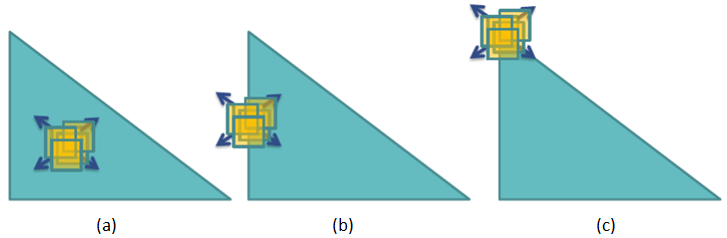
\includegraphics[width=0.55\textwidth]{fig/6.png}
    \vspace{-1em}   
    \begin{center}    
    \caption{\textcolor{gray}{\footnotesize \textit{
     Tre udvalgte vinduer, med interessepunkter i centrum af samme motiv. \textbf{(a)} Punktet er lokaliseret i en teksturløs region, d.v.s. ingen teksturskift. \textbf{(b)} Punktet er lokaliseret på en kant. \textbf{(c)} Punktet er lokaliseret på et hjørne }}}
    \label{fig:2}
     \end{center}
    \vspace{-2.7em}  
  \end{figure}  
\noindent
En intuitiv måde at definere hvorfor et hjørne er interessant, er at placere et rektangulært vindue omkring punktet. Dette vindue forskydes lokalt i x og y retningen. Opstår der et nyt objekt, identisk med interessepunktet, som resultat af forskydningen er punktet ikke distinktivt og derfor ej interessant. I figur \ref{fig:2} ses tre udvalgte punkter med et rektangulært vindue placeret over. I stil med ovenstående definition, forskydes det firkantede vindue i alle retninger. Forskydes \textbf{(a)} vil det ligne alle de forskudte billeder da punktet og regionen omkring er homogent. Punktet er derfor ikke interessant. Forskydes \textbf{(b)} i x-aksen opnås et nyt objekt, men en forskydning i y-aksen vil resultere i samme objekt af en kant, og punktet er derfor ikke interessant. Punktet placeret på et hjørne \textbf{(c)} er interessant da ingen forskydninger vil resultere i det originale billedet. Hjørnet kan derfor bruges som et interessepunkt. Denne intuitive definition kan kvantificeres til en matematisk definition, der estimere auto-korrelationen imellem de forskudte billeder, hvilket angiver intensitetsskiftene imellem billederne og derved, hvor der opstår et hjørne. 